With our dual ablation system, we can reliably co-trap carbon and beryllium ions and introduce cold molecules from the CBGB. Introducing water entrained in a cold neon buffer gas beam, we can see the reaction products due to these collisions. The internal temperature of the buffer gas in the beam is verified to be, which is defined by the temperature of the inner cell.

We do not expect any reactions to occur with the cold neon buffer gas. We have experimentally verified the absence of new mass peaks when introducing neon into the system with carbon and beryllium ions, only an overall loss rate attributed to elastic collisions within the trap. \todo{Add graphs of fluorescence decay}

\begin{figure}[H]
	\centering
	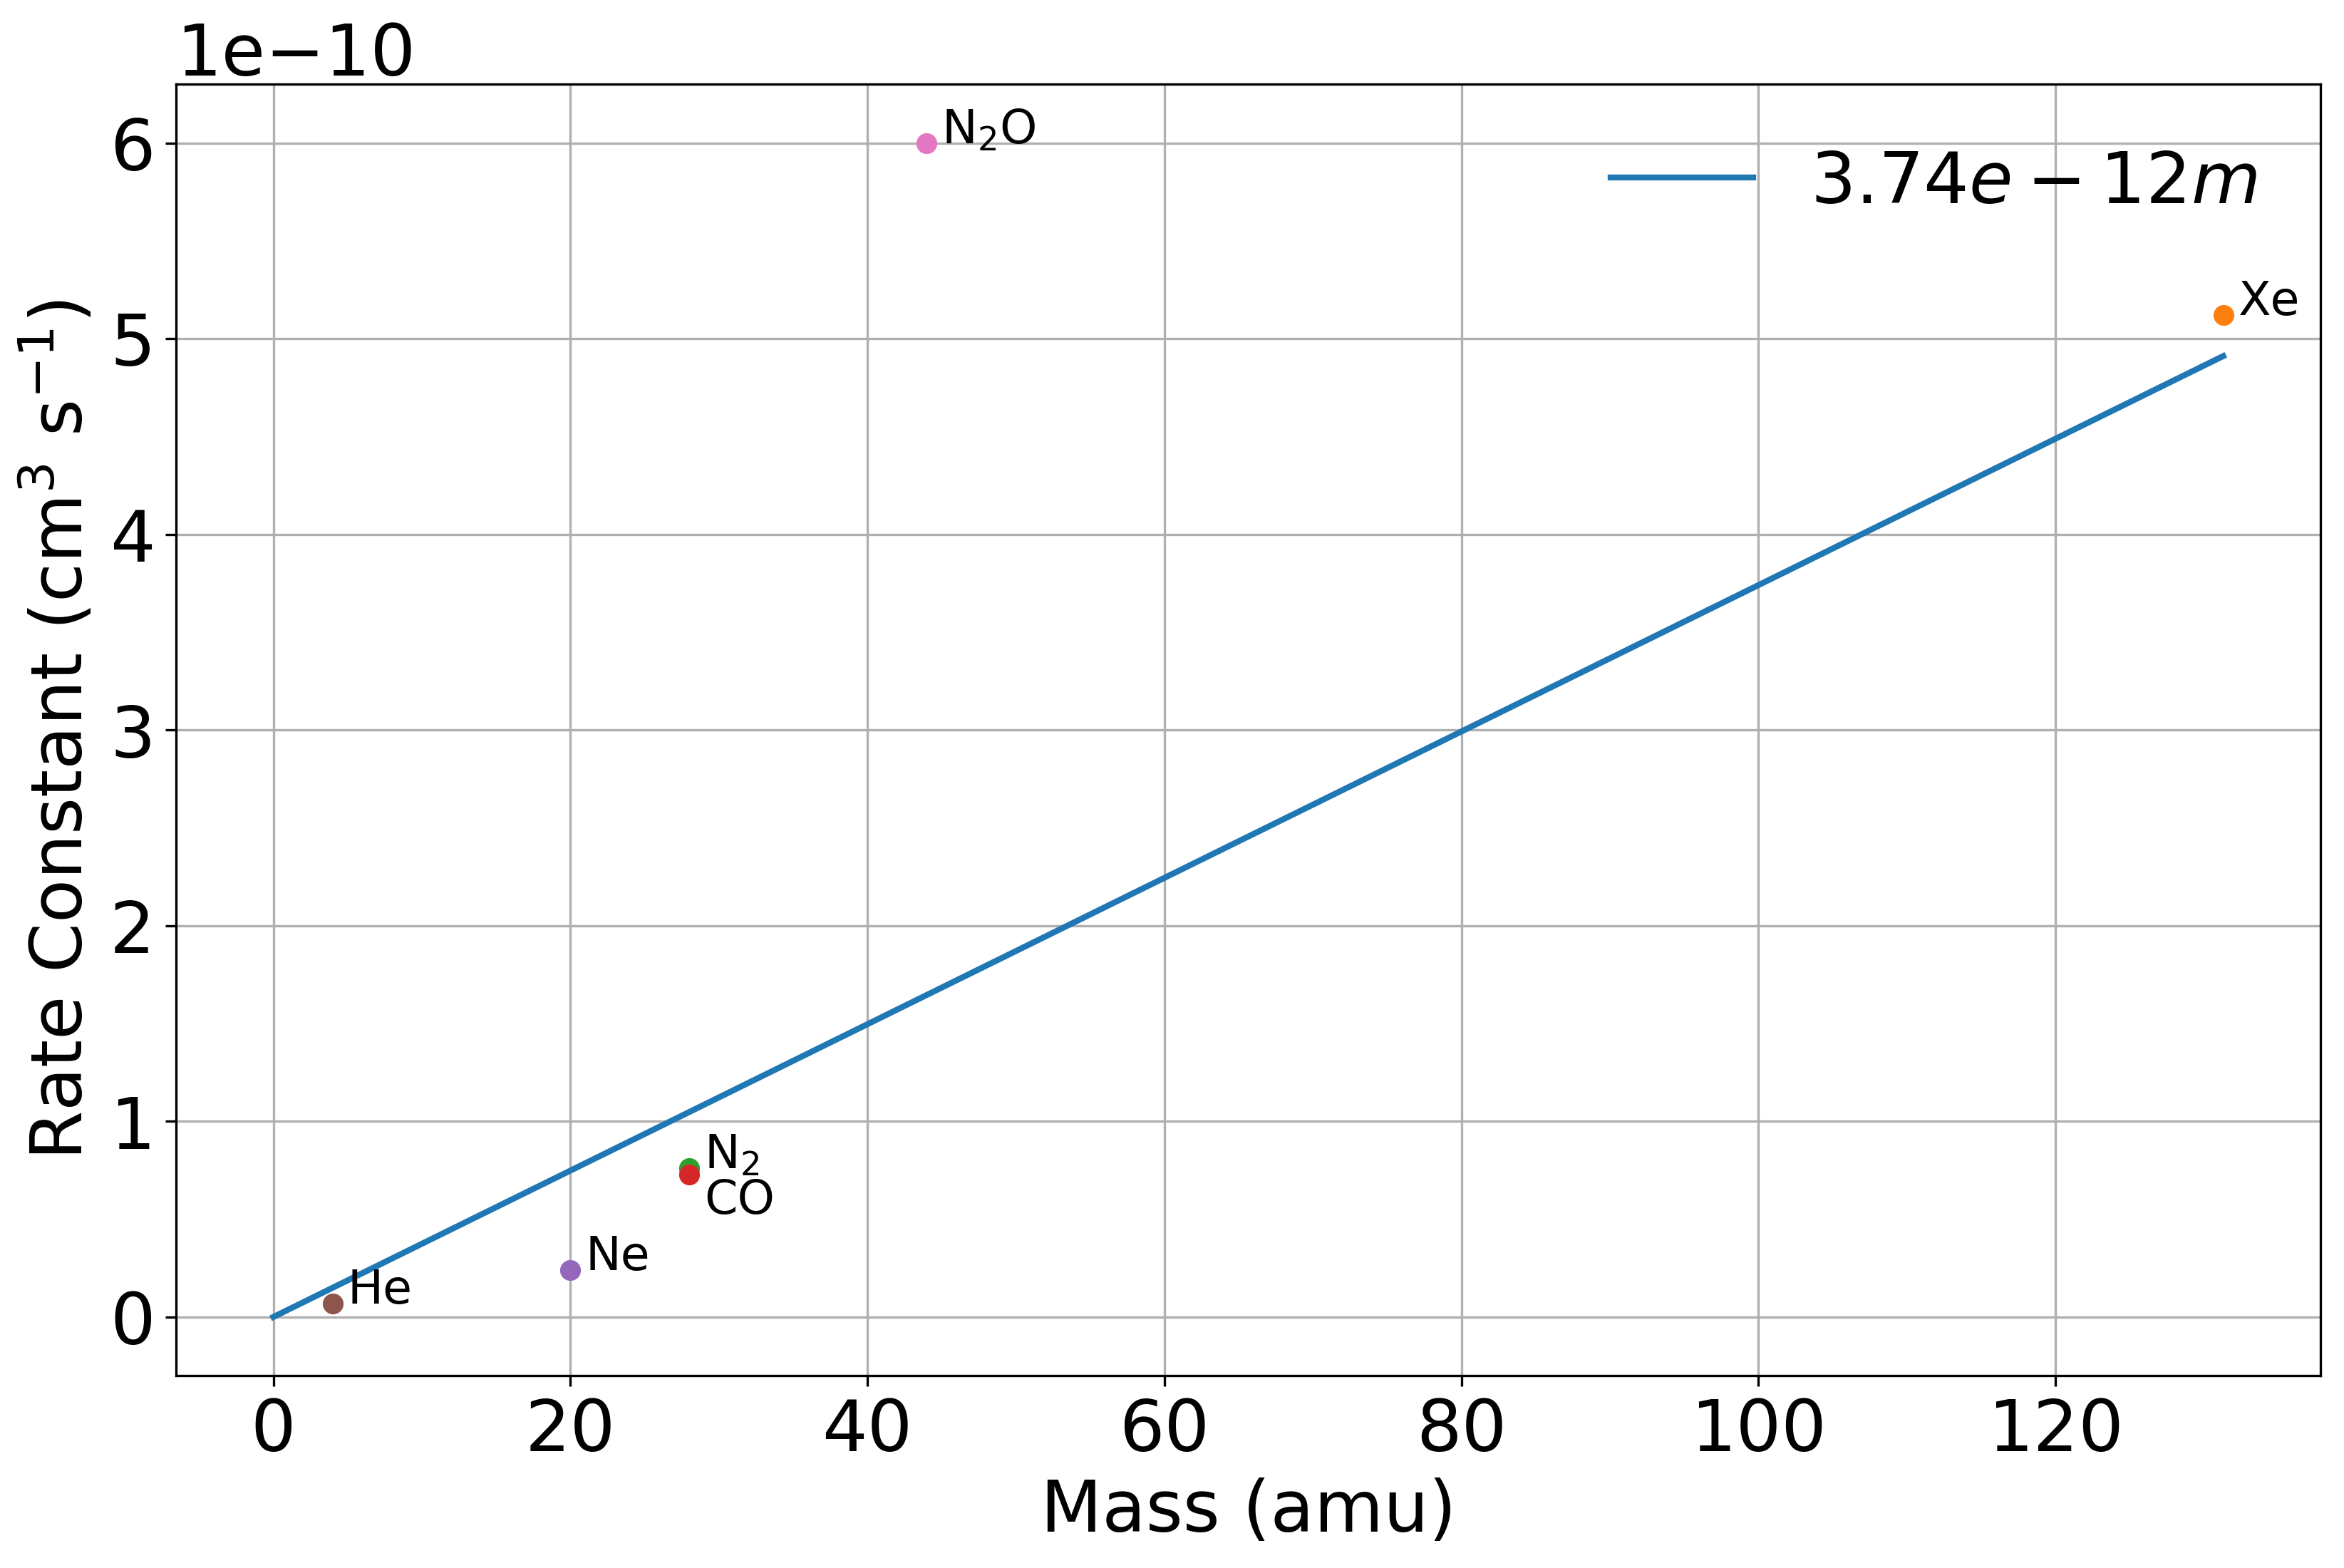
\includegraphics[width=0.8\textwidth]{images/Be_noble_gasses.png}
	\caption{Gasses}
	\label{fig: Be noble gasses}
\end{figure}

Conversely, the water molecules will react readily with both beryllium and carbon ions, where the prevailing beryllium reactions are \cref{r: Be(S)+H2O->BeOH,r: Be(P)+H2O->BeOH,r: Be(P)+H2O->H2O}. Considering the known reaction products of \ce{C+ + H2O}:

\begin{align}
	\ce{C+ + H2O & -> HCO+ + H} \label{r: C+H2O->HCO} \\
	\ce{& -> COH+ + H} \label{r: C+H2O->COH} \\
	\ce{[HCO]+ + H2O & -> H3O+ + CO} \label{r: [HCO]+H2O->H3O}
\end{align}

\begin{align}
	\ce{C}(t) & = \ce{C0} e^{-k_1 \rho t} \label{eq: C(t)+H2O} \\
	\ce{[HCO]}(t) & = \frac{e^{-(k_1 + k_2) \rho t}}{k_1 - k_2} \left(e^{k_1 \rho t}((\ce{C0} + \ce{[HCO]0})k_1 - \ce{[HCO]0} k_2) - \ce{C0} e^{-(k_1 + k_2) \rho t}\right) \label{eq: C+H2O->[HCO](t)} \\
%	H_3O(t) & = \frac{\left([HCO]_0 e^{-k_2 \rho t} - (H_3O_0 + [HCO]_0) \right)(k_2 - k_1) + C_0\left( k_1 \left(1 - e^{-k_2 \rho t}\right) + k_2 \left(e^{-k_1 \rho t} - 1\right) \right)}{k_1 - k_2} \label{eq: [HCO]+H2O->H3O(t)}
	\ce{H3O}(t) & = \ce{H3O0} + \ce{[HCO]0} (1 - e^{-k_2 \rho t}) + \frac{\ce{C0}\left( k_1 \left(1 - e^{-k_2 \rho t}\right) + k_2 \left(e^{-k_1 \rho t} - 1\right) \right)}{k_1 - k_2} \label{eq: [HCO]+H2O->H3O(t)}
\end{align}

We want to probe the branching ratio of the formyl isomers formed in reactions \ref{r: C+H2O->HCO} and \ref{r: C+H2O->COH} at low temperatures. At room temperatures, the branching ratio has been found to be approximately 84:16 (\ce{COH+}:\ce{HCO+})\cite{Freeman1987}, but unexplored at lower regimes.

By definition, these formyl isomers of reactions \cref{r: C+H2O->HCO,r: C+H2O->COH} have identical mass and thus, cannot be readily read off by the TOF system. To be able to separate the isomer products, we need to be able to separate their masses. By introducing a gas into the system with a proton affinity in between the isomer products, we may selectively react only one the less stable \ce{COH+} isomer. This also yields a distinct $m/z$ peaks due to each isomer. By using an external gas, we are doing an indirect measurement, and as such, it may add unintended complications. Certain gasses are more reactive and may react with the excited \ce{Be+}, \ce{C+}, or any other ionized species in the trap. Another possibility is that the \ce{COH+} may isomerize due to interactions with the gas(\ref{r: X+COH->XH}).\cite{Love1987}

\begin{align}
	\ce{COH+ + X & -> XH+ + CO} \label{r: X+COH->XH} \\
	\ce{& -> HCO+ + X} \label{r: X+COH->HCO} \\
	\ce{HCO+ + X & -> no reaction} \label{r: X+HCO->NR}
\end{align}

\begin{table}[H]
	\centering
	\label{t: affinities}
	\begin{tabular}{|l|c|}
	\hline
 & Affinity (kcal/mol)   \\
 \hline
	\ce{CO}* & 427               \\
	\ce{Kr}  & 425               \\
	\ce{HF}  & 490               \\
	\ce{N2}  & 495               \\
	\ce{Xe}  & 496               \\
	\ce{NO}  & 531               \\
	\ce{CO2} & 548               \\
	\ce{CH4} & 552               \\
	\ce{HCl} & 564               \\
	\ce{HBr} & 569               \\
	\ce{N2O} & 571               \\
	*\ce{CO} & 594 \\
	\hline
	\end{tabular}
	\caption{Proton affinities of gasses between formyl isomers where (*) indicates H bonding location.}
\end{table}

Previous literature utilized gasses such as \ce{NO}, \ce{CH4}, \ce{N2O}, and \ce{Kr} to perform similar titrations. \ce{Kr}, and \ce{Xe} are inert and would not react with any other trapped ion but are too heavy to reliably trap after a reaction. \ce{NO} is caustic and will ruin the vacuum chamber if introduced, and thus was avoided. Attempts were make with \ce{N2O} and well as \ce{CH4}, but both had issues. \ce{N2O} rapidly reacts with \ce{Be+} and made reliable TOF traces unattainable due to the loss of coolant ion. \ce{CH4} readily reacted with most of the ions in the trap to produce a multitude of mass peaks, greatly complicating the analysis. At the end, success was found with \ce{CO2} and \ce{^{15}N2}.
